\section{问题一：给定镜场的光学性能评价}

\subsection{问题分析与建模主线}

问题一并非只需把题面给出的五项效率代入乘积公式。余弦效率取决于每面镜的三维姿态，阴影与遮挡取决于光线在反射前后的有向路径，截断效率又取决于太阳并非单一平行方向以及接收器具有有限尺寸。因此，必须先定义从太阳辐射到圆柱接收器接收能量的连续物理映射，再选择数值方法求解其中的几何积分。

本问固定吸收塔平面坐标为$(0,0)$，按修订几何口径取集热器中心为$(0,0,76)$ m。附件给出1745面定日镜的镜心平面坐标；每面镜为$6\ \mathrm{m}\times6\ \mathrm{m}$，镜心高度均为4 m，总采光面积为$62820\ \mathrm{m^2}$。题目规定每月21日的9:00、10:30、12:00、13:30和15:00作为代表时点，故评价集合共有$12\times5=60$个状态。

图\ref{fig:q1-workflow}先给出本问的完整建模链。图中左栏回答“每一步计算什么”，右栏紧接着回答“为什么必须先做这一步”；左栏纵向箭头表示前一步是后一步的输入或定义基础，最下方虚线框才表示数值求解层。低差异采样、GPU分块和采样数只用于近似求解已经定义的连续积分，不参与定义太阳角、阴影、遮挡或截断效率。

\begin{figure}[H]
  \centering
  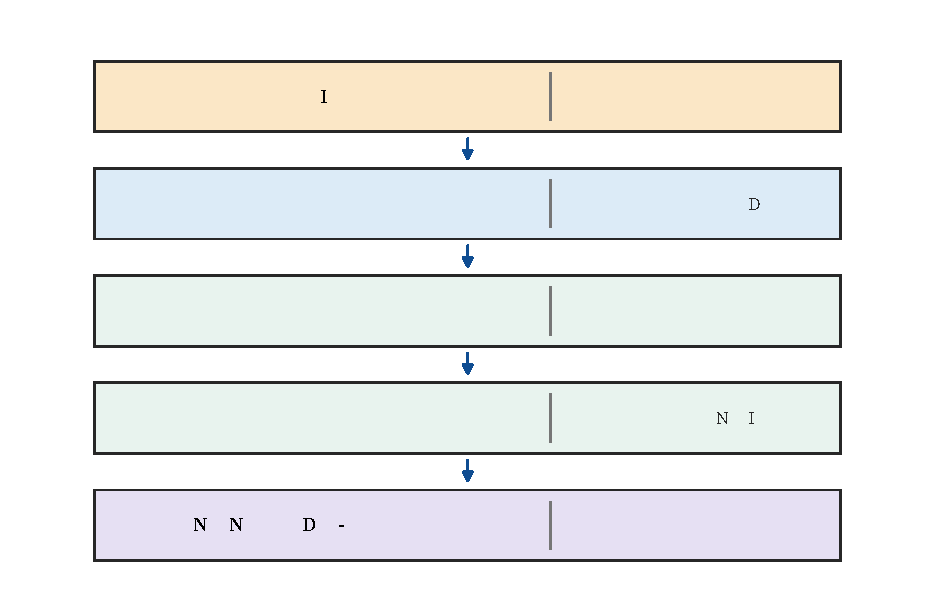
\includegraphics[width=0.98\textwidth]{figures/q1_model_workflow_cn.pdf}
  \caption{问题一各建模步骤、采用原因及数值求解边界}
  \label{fig:q1-workflow}
\end{figure}

由图\ref{fig:q1-workflow}可见，本问按“太阳输入$\rightarrow$镜面几何$\rightarrow$联合样本$\rightarrow$有向光路事件$\rightarrow$条件效率$\rightarrow$逐状态功率与聚合”的顺序建模。每一步都解决下一步的必要前提：太阳方向统一全部光学输入，有限镜面使相交事件可定义，联合样本保证各项损失针对同一份能量，条件截断保证效率乘积符合能量守恒，逐状态功率则保留DNI与效率的同步变化。因此，流程不是计算模块的简单罗列，而是一条不能任意交换顺序的物理推导链。

\subsection{坐标系、基本假设与适用范围}

建立右手直角坐标系：$x$轴向东，$y$轴向北，$z$轴竖直向上。太阳方位角从正北顺时针量取。按本文采用的几何口径，塔身是半径3.5 m、$0\le z<72$ m的实体圆柱；集热器侧面为半径3.5 m、$72\le z\le80$ m的有限圆柱侧面，中心为$(0,0,76)$。阴影表示入射光到达目标镜之前被其他镜面或塔身截断，遮挡表示反射光到达接收器区域之前被其他镜面截断；同一条光线即使与多个物体相交，也只记一次损失。

在题面没有给出额外参数的部分，采用以下经确认的简化：定日镜为理想平面镜，不加入面形误差、斜率误差和跟踪误差；太阳锥采用半角$\theta_\odot=4.65\times10^{-3}$ rad的均匀pillbox太阳盘；五个时点等权形成月平均，十二个月等权形成题面离散年平均；到达圆柱侧面的反射能量按题面公式全部计入输出热功率，不再擅自乘入接收器吸收率。

因此，后文“年平均”专指60个规定状态的等权离散平均，不是逐日逐小时气象积分；所得光学性能也只对应理想平面镜和均匀pillbox太阳盘，不直接等同于包含污染、跟踪误差和热损失的实际电站年发电量。

\subsection{步骤一：由规定时点确定太阳位置与DNI}

令状态集合为
\begin{equation}
\mathcal{T}=\left\{(m,h):m=1,\ldots,12;\ h\in\{9,10.5,12,13.5,15\}\right\}.
\end{equation}
对$t=(m,h)\in\mathcal{T}$，记每月21日相对春分的天数为$D_m$，当地纬度为$\varphi=39.4^\circ$。根据题面附录，赤纬角、时角与高度角依次满足
\begin{equation}
\sin\delta_m=\sin\left(\frac{2\pi D_m}{365}\right)\sin 23.45^\circ,
\qquad \omega_h=\frac{\pi}{12}(h-12),
\end{equation}
\begin{equation}
\sin\alpha_s(t)=\cos\delta_m\cos\varphi\cos\omega_h+
\sin\delta_m\sin\varphi.
\end{equation}

题面只给出方位角余弦，反余弦本身不能区分上午和下午。先计算
\begin{equation}
C_\gamma(t)=\frac{\sin\delta_m-\sin\alpha_s(t)\sin\varphi}
{\cos\alpha_s(t)\cos\varphi},
\end{equation}
再利用时角补足象限：
\begin{equation}
\gamma_s(t)=
\begin{cases}
\arccos C_\gamma(t), & \omega_h\le 0,\\
2\pi-\arccos C_\gamma(t), & \omega_h>0.
\end{cases}
\end{equation}
这样定义后，上午太阳位于东侧，下午位于西侧，正午位于南侧。镜场指向太阳中心的单位向量为
\begin{equation}
\boldsymbol{s}(t)=
\begin{bmatrix}
\cos\alpha_s(t)\sin\gamma_s(t)\\
\cos\alpha_s(t)\cos\gamma_s(t)\\
\sin\alpha_s(t)
\end{bmatrix}.
\end{equation}

太阳高度角和方位角分别控制太阳方向的铅垂分量与水平投影。图\ref{fig:q1-solar-geometry}把三维方向拆成水平面和铅垂面两个视图，以明确方位角从正北顺时针的约定和高度角相对于地平面的定义。

\begin{figure}[H]
  \centering
  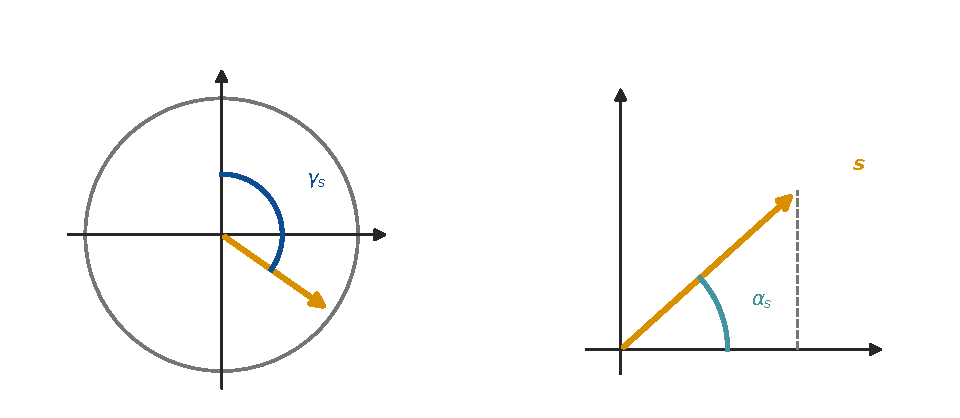
\includegraphics[width=0.94\textwidth]{figures/q1_solar_geometry_cn.pdf}
  \caption{太阳高度角、方位角及太阳中心向量的坐标约定}
  \label{fig:q1-solar-geometry}
\end{figure}

图\ref{fig:q1-solar-geometry}(a)解释了为何方位角必须结合时角确定象限；图\ref{fig:q1-solar-geometry}(b)说明$\sin\alpha_s$就是太阳单位向量的竖直分量。太阳向量既用于后续镜面姿态和阴影光路，也出现在DNI公式中，因此太阳角是整个模型的第一项承重输入。

题目给定海拔$H=3$ km，代入附录参数后，法向直接辐射辐照度为
\begin{equation}
\mathrm{DNI}(t)=1.366\left[0.34981+0.5783875
\exp\left(-\frac{0.275745}{\sin\alpha_s(t)}\right)\right]\ \mathrm{kW/m^2}.
\end{equation}
$\mathrm{DNI}$给出垂直于太阳中心光线平面的能量通量，$\boldsymbol{s}$给出光线方向。余弦效率将在镜面上完成投影，因此不能把DNI再乘一次水平面投影因子。

在把60个状态输入镜场模型之前，需要确认它们都是有效白昼状态，并检查季节和时刻变化是否符合球面几何。图\ref{fig:q1-solar-states}分别给出60个状态的太阳高度角和DNI；每个单元格都对应后续全场计算中的一个时点。

\begin{figure}[H]
  \centering
  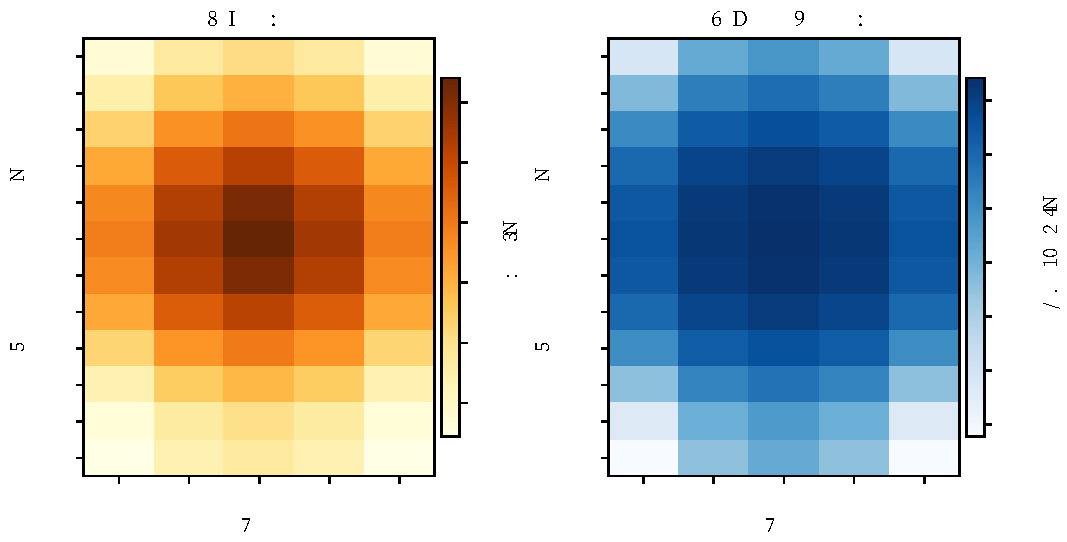
\includegraphics[width=0.98\textwidth]{figures/q1_solar_states_cn.pdf}
  \caption{题目规定60个状态的太阳高度角与法向直接辐射辐照度}
  \label{fig:q1-solar-states}
\end{figure}

图\ref{fig:q1-solar-states}表明60个状态的太阳高度角和DNI均为正；同月内正午最高，同一时刻由冬季向夏季整体升高。上午和下午关于正午具有相同的高度角与DNI，但方位角处于不同象限，所以镜场空间损失仍可能不同，不能只凭DNI对称性推断镜场效率完全对称。

\subsection{步骤二：由反射定律确定镜面姿态}

第$i$面镜的镜心为$\boldsymbol{c}_i=(x_i,y_i,4)^{\mathsf T}$，集热器中心为$\boldsymbol{c}_R=(0,0,76)^{\mathsf T}$。镜心指向集热器中心的单位向量为
\begin{equation}
\boldsymbol{t}_i=\frac{\boldsymbol{c}_R-\boldsymbol{c}_i}
{\|\boldsymbol{c}_R-\boldsymbol{c}_i\|}.
\end{equation}
太阳中心光线的传播方向是$-\boldsymbol{s}$。理想镜面反射算子为
\begin{equation}
\mathcal{R}(\boldsymbol{d},\boldsymbol{n})
=\boldsymbol{d}-2(\boldsymbol{d}\cdot\boldsymbol{n})\boldsymbol{n}.
\end{equation}
控制规则要求$\mathcal{R}(-\boldsymbol{s},\boldsymbol{n}_i)=\boldsymbol{t}_i$，由入射方向与目标方向的角平分关系得到唯一朝阳法向
\begin{equation}
\boldsymbol{n}_i(t)=\frac{\boldsymbol{s}(t)+\boldsymbol{t}_i}
{\|\boldsymbol{s}(t)+\boldsymbol{t}_i\|}.
\end{equation}
该式给出的不是固定安装角，而是随太阳位置更新的目标姿态。对固定的第$i$面镜，$\boldsymbol{t}_i$在一天内保持不变；每到一个计算时点，先更新$\boldsymbol{s}(t)$，再由上式更新$\boldsymbol{n}_i(t)$。因此，同一面镜上午、正午和下午需要转到不同姿态；同一时点的不同镜面也因$\boldsymbol{t}_i$不同而具有不同姿态。

为直观表示控制角，定义法向方位角$\beta_i$从正北顺时针量取，镜面倾角$\tau_i$为镜面平面相对水平面的夹角，则
\begin{equation}
\beta_i(t)=\operatorname{mod}\!\left[
\operatorname{atan2}\bigl(n_{x,i}(t),n_{y,i}(t)\bigr),2\pi\right],
\qquad
\tau_i(t)=\arccos n_{z,i}(t).
\end{equation}
当$\tau_i=0$时镜面水平。这两个角确定题面模型中的目标镜面平面；实际电机轴角还依赖支架零位和传动形式，题面没有提供，故不另行虚构。

以附件第1面镜$\boldsymbol{c}_1=(107.25,11.664,4)^{\mathsf T}$ m为例，图\ref{fig:q1-single-tracking}给出3月21日五个时点的目标姿态。该镜位于塔的东偏北侧，因此即使上午、下午太阳高度角关于正午对称，其镜面姿态也不必关于正午对称。
\begin{figure}[H]
  \centering
  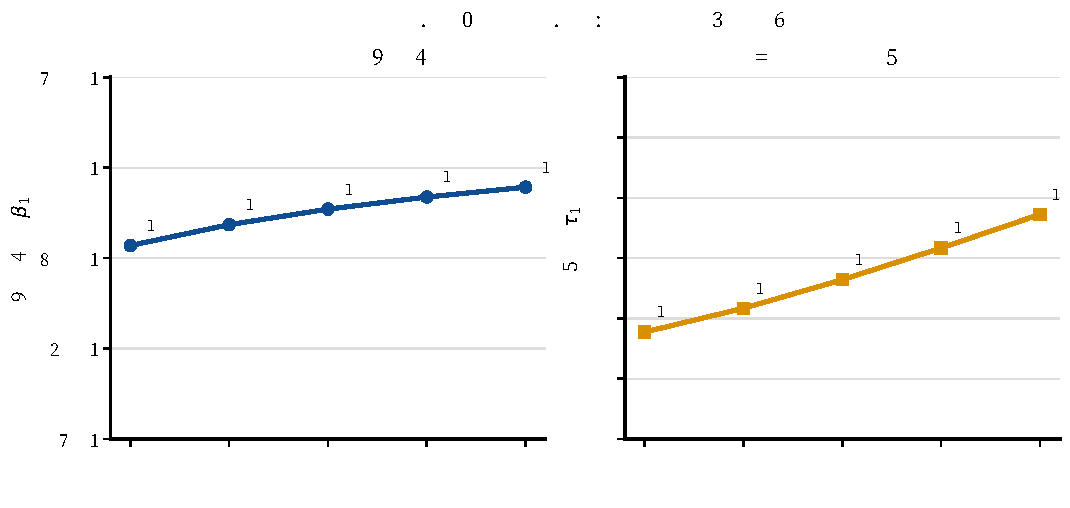
\includegraphics[width=0.92\textwidth]{figures/q1_single_mirror_tracking_cn.pdf}
  \caption{附件第1面定日镜在3月21日的时变目标姿态}
  \label{fig:q1-single-tracking}
\end{figure}

这里“使光线尽量反射至集热器”严格对应题面中心瞄准规则：太阳盘中心光线经镜心反射后指向集热器中心。它不是额外的瞄准点优化，也不意味着太阳锥中的所有边缘光线都必然命中有限接收器；后者仍由截断效率计算。

因此余弦效率是反射几何的解析结果：
\begin{equation}
\eta_{\cos,i}(t)=\boldsymbol{n}_i(t)\cdot\boldsymbol{s}(t)
=\sqrt{\frac{1+\boldsymbol{s}(t)\cdot\boldsymbol{t}_i}{2}}.
\end{equation}

法向只确定镜面所在平面，尚未给出有限矩形边界。令$\boldsymbol{k}=(0,0,1)^{\mathsf T}$，根据“上下边平行地面”的题意构造
\begin{equation}
\boldsymbol{e}_{w,i}=\frac{\boldsymbol{k}\times\boldsymbol{n}_i}
{\|\boldsymbol{k}\times\boldsymbol{n}_i\|},
\qquad
\boldsymbol{e}_{h,i}=\boldsymbol{n}_i\times\boldsymbol{e}_{w,i}.
\end{equation}
于是有限矩形镜面为
\begin{equation}
\mathcal{M}_i(t)=\left\{\boldsymbol{c}_i+u\boldsymbol{e}_{w,i}(t)
+v\boldsymbol{e}_{h,i}(t):u,v\in[-3,3]\right\}.
\end{equation}

这一步需要同时说明反射方向和镜面边界，因为后续光线相交既依赖法向，又必须检查交点是否真正落在$6\ \mathrm{m}\times6\ \mathrm{m}$矩形内部。图\ref{fig:q1-reflection}左图表示法向的角平分关系，右图表示局部宽向、高向和法向如何共同参数化有限镜面。

\begin{figure}[H]
  \centering
  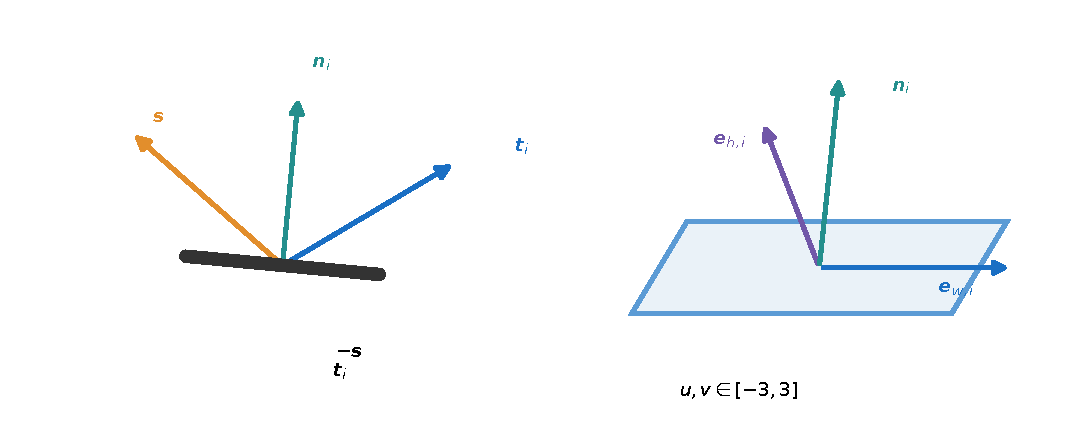
\includegraphics[width=0.98\textwidth]{figures/q1_reflection_geometry_cn.pdf}
  \caption{镜面反射方向、唯一法向与有限矩形局部坐标}
  \label{fig:q1-reflection}
\end{figure}

图\ref{fig:q1-reflection}(a)与法向公式对应：$\boldsymbol{n}_i$位于指向太阳的方向$\boldsymbol{s}$和指向接收器的方向$\boldsymbol{t}_i$之间；图\ref{fig:q1-reflection}(b)与有限镜面参数式对应：只有同时满足$u,v\in[-3,3]$的交点才位于真实镜面上。至此，太阳位置被转换成每个时点、每面镜的唯一三维有限几何对象。

\subsection{步骤三：建立太阳盘方向测度}

题面指出太阳光具有锥形角，说明太阳不能被视为严格单一方向。由于题面没有给出周日比或现场太阳形状，采用经确认的半角$\theta_\odot=4.65\times10^{-3}$ rad均匀pillbox太阳盘。在$\boldsymbol{s}$的正交平面内构造单位基$\boldsymbol{a},\boldsymbol{b}$，太阳盘内方向表示为
\begin{equation}
\boldsymbol{s}'(t,\theta,\psi)=\boldsymbol{s}(t)\cos\theta+
\left[\boldsymbol{a}(t)\cos\psi+\boldsymbol{b}(t)\sin\psi\right]\sin\theta,
\end{equation}
其中$0\le\theta\le\theta_\odot$，$0\le\psi<2\pi$。均匀pillbox是单位立体角内能量相同，因此归一化方向测度为
\begin{equation}
\mathrm{d}\mu_s=\frac{\sin\theta\,\mathrm{d}\theta\,\mathrm{d}\psi}
{2\pi(1-\cos\theta_\odot)}.
\end{equation}
数值采样必须使$\cos\theta$均匀，而不能使$\theta$均匀；否则会过度采样太阳盘中心，系统改变接收器边界附近的命中比例。

镜面法向仍由太阳中心方向确定，但太阳盘内每个方向都要逐条反射：
\begin{equation}
\boldsymbol{r}'_i=-\boldsymbol{s}'+2(\boldsymbol{s}'\cdot\boldsymbol{n}_i)\boldsymbol{n}_i.
\end{equation}
只有$\boldsymbol{s}'=\boldsymbol{s}$时，反射方向才严格等于$\boldsymbol{t}_i$。因此，中心光线命中接收器中心并不能替代对整个太阳锥的有限接收器命中计算。

\subsection{步骤四：在统一光线上定义阴影、遮挡和截断}

对第$i$面镜和时点$t$，定义联合样本空间
\begin{equation}
\Omega_i(t)=\mathcal{M}_i(t)\times\mathcal{S}(t),
\qquad \mathrm{d}\mu_i=\frac{\mathrm{d}A}{A_i}\,\mathrm{d}\mu_s,
\quad A_i=36\ \mathrm{m^2}.
\end{equation}
一个样本$\xi=(\boldsymbol{p},\boldsymbol{s}')$同时指定镜面位置和太阳盘方向，代表一小份确定光路的能量。阴影、遮挡和截断均在同一个联合样本空间上判断，才能保证损失分母一致。

入射阶段从镜面点朝太阳方向回溯：
\begin{equation}
\boldsymbol{q}_{\mathrm{in}}(\lambda)=\boldsymbol{p}+\lambda\boldsymbol{s}',\qquad\lambda>0.
\end{equation}
先定义塔身实体区域
\begin{equation}
\mathcal{C}_T=\{(x,y,z):x^2+y^2\le3.5^2,\ 0\le z<72\}.
\end{equation}
若入射射线不与任何其他有限镜面相交，令$J_i(\xi)=1$，否则为0；若它不与$\mathcal{C}_T$相交，令$T_i(\xi)=1$，否则为0。于是联合入射可见指示量为
\begin{equation}
I_i(\xi)=J_i(\xi)T_i(\xi).
\end{equation}
这样，镜间阴影和塔身阴影在同一条光线上作布尔合并，不会重复扣损。按建模者确认的口径，$72\le z\le80$ m的集热器不作为入射阴影体；该区间只在反射后的接收命中判定中使用。出射阶段沿反射方向追踪
\begin{equation}
\boldsymbol{q}_{\mathrm{out}}(\lambda)=\boldsymbol{p}+\lambda\boldsymbol{r}'_i,\qquad\lambda>0.
\end{equation}
若反射光在到达接收器区域之前先与其他镜面相交，则发生遮挡。定义出射可见指示量$O_i(\xi)$：未被遮挡时取1，否则取0。

阴影和遮挡发生在反射前后不同的有向光段。图\ref{fig:q1-shadow-blocking}分别给出两类光路，以避免把它们混作无方向的平面重叠面积。

\begin{figure}[H]
  \centering
  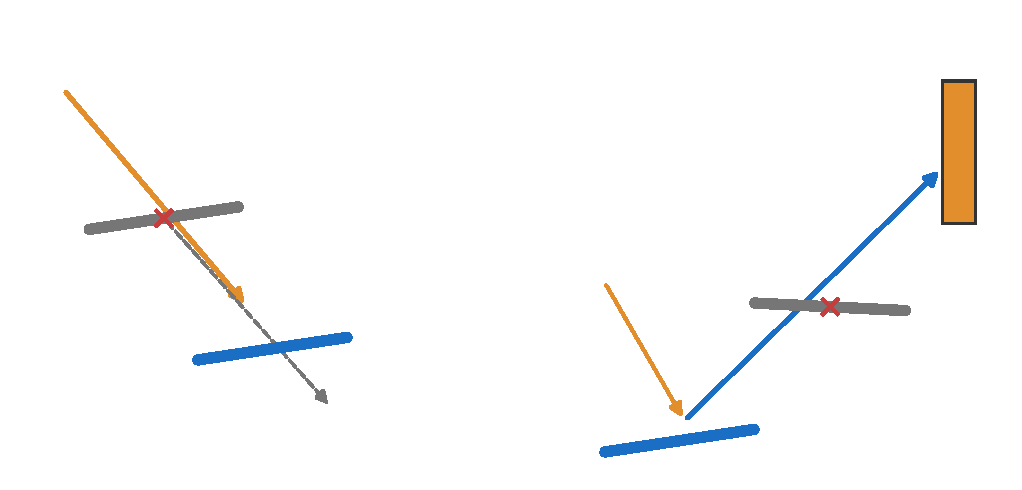
\includegraphics[width=0.98\textwidth]{figures/q1_shadow_blocking_cn.pdf}
  \caption{入射阴影与出射遮挡的有向光路区别}
  \label{fig:q1-shadow-blocking}
\end{figure}

图\ref{fig:q1-shadow-blocking}(a)中光线尚未到达目标镜就与邻镜或塔身相交；图\ref{fig:q1-shadow-blocking}(b)中太阳光已到达目标镜，但反射后在到达接收器前与邻镜相交。程序因此分别沿$+\boldsymbol{s}'$和$+\boldsymbol{r}'$检查正向射线参数，不能用同一个反向投影公式代替两类事件。

接收器有效受光面为
\begin{equation}
\mathcal{C}=\{(x,y,z):x^2+y^2=R^2,\ 72\le z\le80\},\qquad R=3.5\ \mathrm{m}.
\end{equation}
将出射射线代入圆柱方程，得到$a\lambda^2+b\lambda+c=0$，其中
\begin{equation}
a=r_x'^2+r_y'^2,\quad
b=2(p_xr_x'+p_yr_y'),\quad
c=p_x^2+p_y^2-R^2.
\end{equation}
取最小正根$\lambda_R$，再检查$p_z+\lambda_Rr_z'\in[72,80]$。满足时定义命中指示量$H_i(\xi)=1$，否则为0。题面指定外表受光式圆柱，故顶面和底面不计入接收面。

截断损失同时来自太阳盘方向展开和接收器有限直径、高度。图\ref{fig:q1-suncone}先说明太阳盘是一族方向，再说明这族反射光中只有部分命中有限圆柱侧面。

\begin{figure}[H]
  \centering
  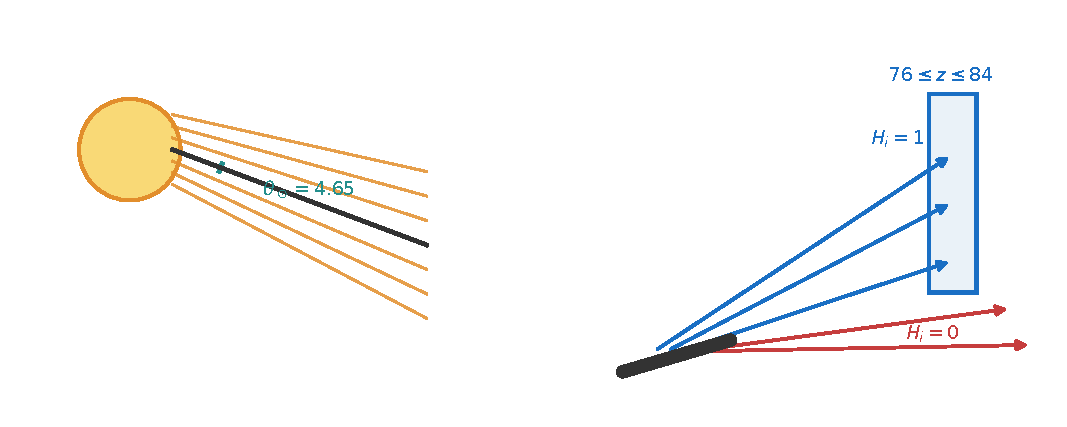
\includegraphics[width=0.98\textwidth]{figures/q1_suncone_receiver_cn.pdf}
  \caption{均匀太阳盘方向与有限圆柱集热器的截断机制}
  \label{fig:q1-suncone}
\end{figure}

图\ref{fig:q1-suncone}(a)对应太阳盘方向测度；图\ref{fig:q1-suncone}(b)对应命中指示量$H_i$。中心光线命中只验证瞄准方向正确，不能说明$\eta_{\mathrm{trunc}}=1$；太阳盘边缘方向和镜面不同位置仍可能形成未命中的反射光。

令光路未受入射阴影和出射遮挡的联合事件为$V_i(\xi)=I_i(\xi)O_i(\xi)$。阴影遮挡效率定义为
\begin{equation}
\eta_{\mathrm{sb},i}(t)=\int_{\Omega_i(t)}V_i(\xi)\,\mathrm{d}\mu_i(\xi).
\end{equation}
题面把截断效率的分母定义为扣除阴影遮挡损失后的反射能量，因此它必须是条件比例：
\begin{equation}
\eta_{\mathrm{trunc},i}(t)=
\frac{\int_{\Omega_i(t)}V_i(\xi)H_i(\xi)\,\mathrm{d}\mu_i(\xi)}
{\int_{\Omega_i(t)}V_i(\xi)\,\mathrm{d}\mu_i(\xi)}.
\end{equation}
于是严格满足
\begin{equation}
\eta_{\mathrm{sb},i}(t)\eta_{\mathrm{trunc},i}(t)
=\int_{\Omega_i(t)}V_i(\xi)H_i(\xi)\,\mathrm{d}\mu_i(\xi).
\end{equation}
右端正是“既未被镜场阻挡，又真正命中接收器”的联合能量比例。该恒等式保证一条光线无论与多少邻镜相交都只记录一次损失，并保证截断效率不使用全部镜面采样作为错误分母。

\subsection{步骤五：从单镜效率到镜场功率}

第$i$面镜到接收器中心的距离为$d_{\mathrm{HR},i}=\|\boldsymbol{c}_R-\boldsymbol{c}_i\|$。附件中全部$d_{\mathrm{HR},i}<1000$ m，故题面大气透射率公式适用：
\begin{equation}
\eta_{\mathrm{at},i}=0.99321-0.0001176d_{\mathrm{HR},i}
+1.97\times10^{-8}d_{\mathrm{HR},i}^2.
\end{equation}
镜面反射率取$\eta_{\mathrm{ref}}=0.92$。单镜综合光学效率为
\begin{equation}
\eta_i(t)=\eta_{\mathrm{sb},i}(t)\eta_{\cos,i}(t)\eta_{\mathrm{at},i}
\eta_{\mathrm{trunc},i}(t)\eta_{\mathrm{ref}}.
\end{equation}
单镜和镜场在时点$t$的输出热功率分别为
\begin{equation}
E_i(t)=\mathrm{DNI}(t)A_i\eta_i(t),
\end{equation}
\begin{equation}
E_{\mathrm{field}}(t)=\sum_{i=1}^{N}E_i(t)
=\mathrm{DNI}(t)\sum_{i=1}^{N}A_i\eta_i(t).
\end{equation}

Q1全部镜面等面积，故时点平均效率可按1745面镜等权：
\begin{equation}
\bar\eta_q(t)=\frac{1}{N}\sum_{i=1}^{N}\eta_{q,i}(t),
\quad q\in\{\mathrm{sb},\cos,\mathrm{trunc},\mathrm{total}\}.
\end{equation}
月平均为当月五个时点的算术平均：
\begin{equation}
\bar\eta_{q,m}=\frac{1}{5}\sum_{h\in\{9,10.5,12,13.5,15\}}\bar\eta_q(m,h),
\end{equation}
题面离散年平均为
\begin{equation}
\bar\eta_{q,\mathrm{year}}=\frac{1}{12}\sum_{m=1}^{12}\bar\eta_{q,m}
=\frac{1}{60}\sum_{t\in\mathcal{T}}\bar\eta_q(t).
\end{equation}

功率也按相同时间权重聚合，但必须先计算每个时点的镜场功率，再求平均：
\begin{equation}
\bar E_{\mathrm{year}}=\frac{1}{60}\sum_{t\in\mathcal{T}}
\mathrm{DNI}(t)\sum_{i=1}^{N}A_i\eta_i(t).
\end{equation}
单位镜面面积年平均输出热功率为
\begin{equation}
P_A=\frac{\bar E_{\mathrm{year}}}{\sum_iA_i}.
\end{equation}
不能用“平均DNI$\times$平均效率”替代上式，因为DNI和光学效率随状态共同变化，两个平均量的乘积一般不等于乘积的平均。

\subsection{连续模型的数值求解}

上述积分包含有限矩形可见性和有限圆柱命中，难以获得闭式解。正式主方法M1分别在镜面局部坐标$(u,v)$和太阳盘立体角上生成随机扰动Sobol低差异样本，再计算两组样本的笛卡尔积。对每个“镜面点--太阳方向”组合依次计算$I_i,O_i,H_i$，用布尔样本均值估计阴影遮挡效率和联合接收比例，最后通过条件关系得到截断效率。

正式细分辨率为64个镜面点与32个太阳方向，共2048条联合光线/镜时种子；固定种子为2023、2024、2025和2026，正式结果取四个细分辨率估计的算术平均。为估计离散误差，同时使用32个镜面点与16个太阳方向的嵌套粗分辨率，相同种子的粗样本是细Sobol序列的前缀。

几何相交只需检查可能影响目标镜的邻镜。程序以镜心平面距离60 m建立候选集，但该剪枝必须与全1745面镜的相交判定进行分层复核。TensorFlow GPU只负责分块执行相同的射线--有限矩形和射线--圆柱求交，不改变物理样本空间或效率定义。

为定位实现错误并量化离散近似影响，另设置可完成全部输出的基线B1。B1在镜面上使用$5\times5$中点网格，以太阳中心方向计算阴影遮挡，再用16个太阳盘方向估计可见网格点的条件截断。B1与M1共享太阳位置、镜面姿态、大气透射、有限圆柱和功率聚合公式，因而二者结果可以直接比较；但B1的低分辨率和因子化近似不用于冻结正式结果。

预定回退规则是：若M1未达到收敛阈值，则将同一方法提高到128个镜面点与64个太阳方向并返回实验判断点；不得把B1自动升级为最终方法。本轮收敛检查通过，故未触发回退。

\subsection{几何验证与数值稳健性}\label{subsec:q1-robustness}

模型验证对应建模链中的具体高风险环节，而不是只检查程序能否运行。除太阳方向、反射方向和集热器命中检查外，还构造了三类塔影案例：入射射线穿过塔身、背离塔身、仅穿过集热器高度区间，预期结果依次为“遮挡、不遮挡、不遮挡”。TensorFlow与NumPy在独立复核案例中的相交计数完全一致；60 m邻镜候选剪枝相对全场判定的阴影遮挡效率最大绝对差为0。

在全部$1745\times60=104700$条逐镜状态记录中，各效率均位于$[0,1]$，未出现NaN或无穷值；联合事件分解的最大残差处于浮点舍入量级，综合效率乘积残差为0，镜场功率与逐镜功率汇总残差为$7.11\times10^{-15}$ MW。这些结果分别验证了太阳角、反射方向、有限边界、条件截断分母和单位聚合。

在把数值写入论文前，还需检查离散分辨率、随机化低差异采样和关键简化假设是否会改变结论。图\ref{fig:q1-robustness}统一使用相对功率变化，并画出预先设置的阈值，避免用截断的绝对功率纵轴夸大小差异。

\begin{figure}[H]
  \centering
  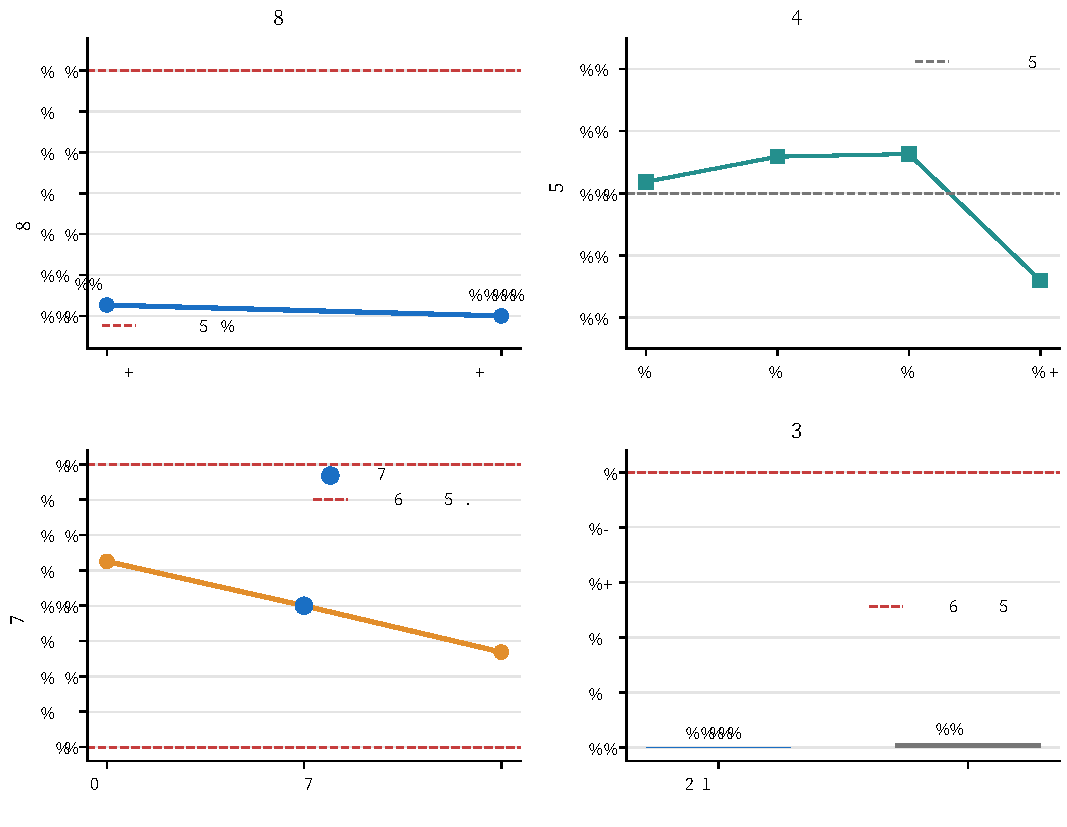
\includegraphics[width=0.98\textwidth]{figures/q1_convergence_robustness_cn.pdf}
  \caption{M1分辨率、固定种子及关键假设的稳健性检查}
  \label{fig:q1-robustness}
\end{figure}

由图\ref{fig:q1-robustness}(a)可见，从$32\times16$提高到$64\times32$后，年平均综合效率的绝对变化为$7.6896\times10^{-5}$，年平均镜场功率相对变化为0.0134\%，12个月单位面积功率的最大相对变化为0.0594\%；三项分别低于0.002、0.3\%和0.5\%阈值。图\ref{fig:q1-robustness}(b)中四种子年平均综合效率标准差为$4.6416\times10^{-5}$，年平均功率极差仅0.007117 MW。

图\ref{fig:q1-robustness}(c)显示，太阳盘半角改变$-5\%$和$+5\%$时，年平均功率分别改变$+0.3140\%$和$-0.3281\%$，均未达到1\%返回决策阈值；太阳锥变宽时反射光斑扩展，功率下降，方向与有限接收器几何一致。图\ref{fig:q1-robustness}(d)显示，按各月天数加权得到34.9918 MW，相对十二个月等权的34.9868 MW仅变化0.0142\%。因此当前分辨率和已批准假设均未触发回退，但这些检查只证明求解器对已定义模型稳定，并不等同于真实电站实测验证。

\subsection{镜场空间分布与月度规律}

全场平均会掩盖不同镜位与太阳时刻的差异。为了说明损失并非一个可对所有镜面套用的常数，图\ref{fig:q1-spatial}先给出附件镜场布局；随后对每面镜的60个规定状态综合效率取等权平均，形成逐镜年均综合光学效率分布；最后选择冬季上午、春季正午和夏季正午三个代表状态展示逐镜瞬时综合效率。年均图与三个时点图使用相同色标，因此既能辨认长期稳定的空间差异，也能直接比较单时点空间不均匀程度。

\begin{figure}[H]
  \centering
  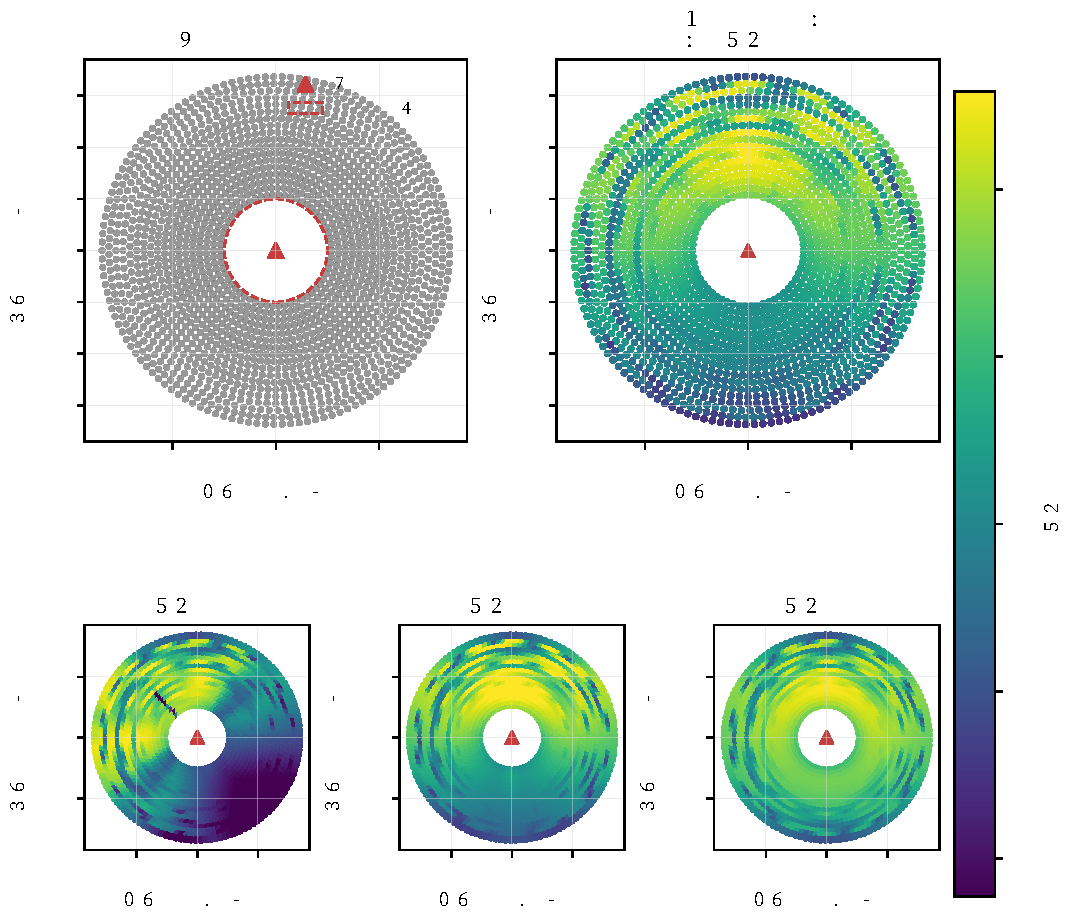
\includegraphics[width=0.98\textwidth]{figures/q1_field_spatial_cn.pdf}
  \caption{镜场布置、逐镜年均综合光学效率与三个代表状态的逐镜综合光学效率}
  \label{fig:q1-spatial}
\end{figure}

图\ref{fig:q1-spatial}(b)给出逐镜年均综合光学效率，它把60个规定状态的短时方向性损失聚合为长期空间差异，可用于识别全年平均意义下持续高效或低效的镜位。图\ref{fig:q1-spatial}(c)表明低太阳高度角下效率具有明显的方向性不均匀，这是余弦方向、镜间遮挡与塔身阴影共同作用的结果；图\ref{fig:q1-spatial}(d)、(e)在正午状态下分布更接近环状，但仍随镜位变化。年均图比单时点更平滑，却没有退化为仅由半径决定的常数，说明必须逐镜、逐时点计算后再聚合，不能只按镜场半径给每面镜赋同一个平均效率。

为把新增的塔身阴影从镜间阴影中单独辨认出来，对第$i$面镜定义60状态累计塔影暴露量
\begin{equation}
N^{\mathrm{eq}}_{T,i}=\sum_{t\in\mathcal{T}}
\Pr_{\boldsymbol{p},\boldsymbol{s}',\mathrm{seed}}
\!\left\{\boldsymbol{q}_{\mathrm{in}}(\lambda)\cap\mathcal{C}_T\neq\varnothing\right\}.
\end{equation}
每个状态中的概率在64个镜面点、32个太阳盘方向和4个固定种子上求平均。因此，$N^{\mathrm{eq}}_{T,i}=1$表示累计塔影暴露量等价于一个规定状态下整面镜完全被塔身遮挡；该量同时反映受影响状态数和每个状态的遮挡面积比例，但不混入镜间阴影。

\begin{figure}[H]
  \centering
  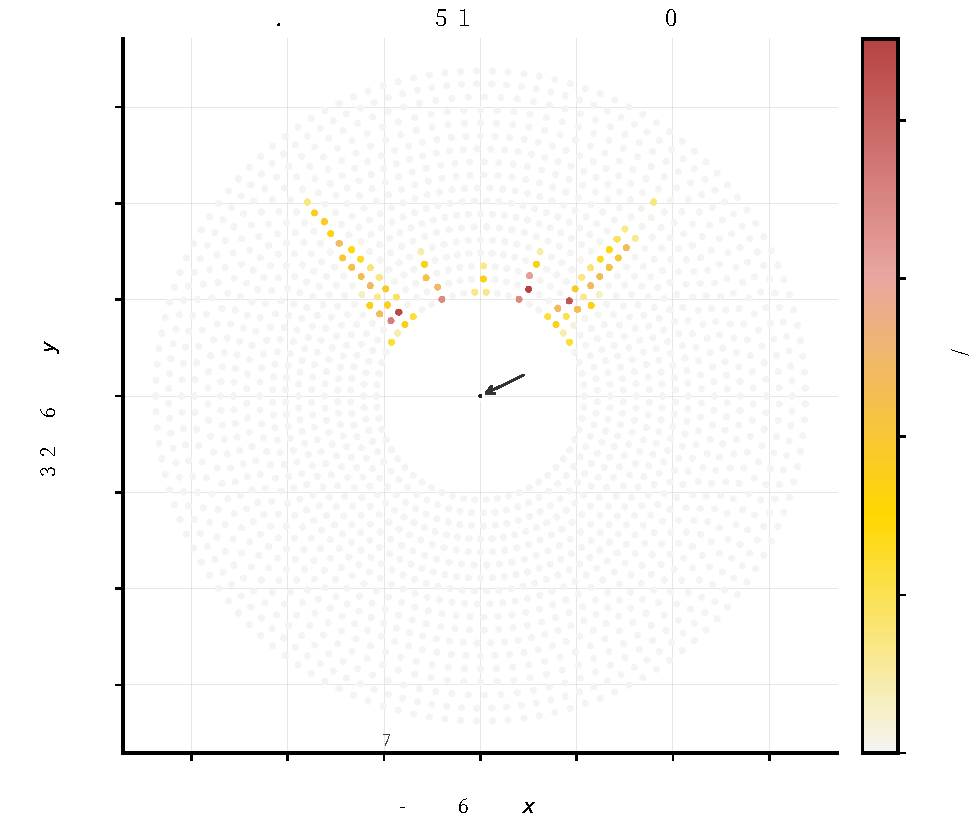
\includegraphics[width=0.92\textwidth]{figures/q1_tower_shadow_exposure_cn.pdf}
  \caption{60个规定太阳状态叠加的定日镜塔身阴影暴露分布}
  \label{fig:q1-tower-shadow}
\end{figure}

图\ref{fig:q1-tower-shadow}中颜色越深，表示累计塔影暴露越强。共有72面定日镜出现非零塔影，单镜最大累计暴露为2.2574个等效状态。受影响镜面主要位于塔的北侧，并向西北和东北展开，这是因为规定时点的太阳位于南侧天空，塔影总体投向北方，而上午、下午太阳方位变化使阴影方向分别发生横向偏转。这里的“全年叠加”特指题目规定60个状态的等权累计，不等同于真实全年逐分钟遮挡时长。

月度功率同时受到DNI、余弦效率、阴影遮挡效率、截断效率和大气透射率影响。因此，图\ref{fig:q1-monthly}左侧同时展示主要效率分量，右侧展示最终单位面积功率，避免把季节变化错误归因于单一因素。

\begin{figure}[H]
  \centering
  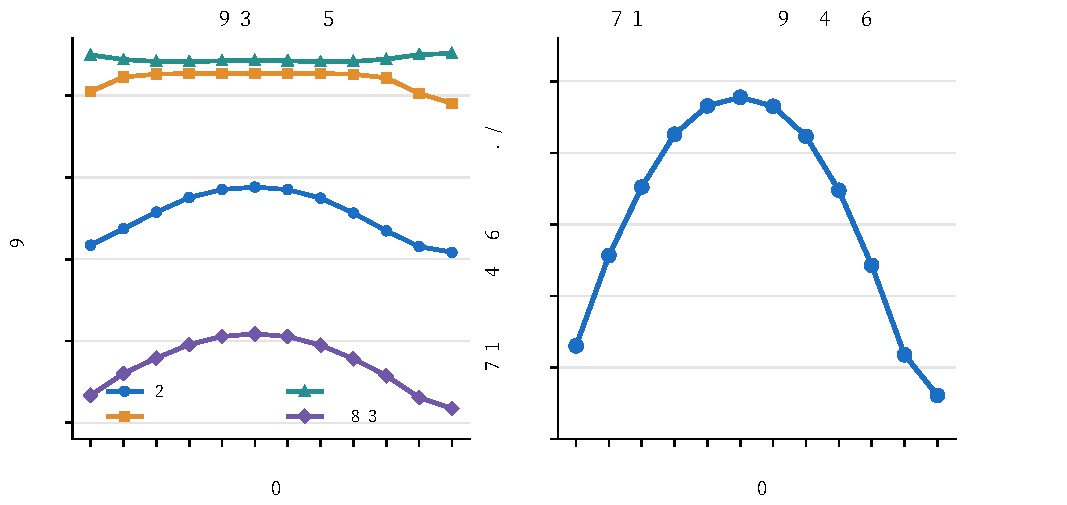
\includegraphics[width=0.98\textwidth]{figures/q1_monthly_results_cn.pdf}
  \caption{月平均光学效率分解与单位镜面面积输出热功率}
  \label{fig:q1-monthly}
\end{figure}

图\ref{fig:q1-monthly}显示，余弦效率和阴影遮挡效率由冬季向夏季上升，再向冬季下降；截断效率全年均高于0.941，变化较小且冬季略高，但不能抵消冬季较低的DNI、余弦效率和阴影遮挡效率。单位面积月平均输出热功率在6月达到最高值0.6388 kW/m$^2$，在12月达到最低值0.4306 kW/m$^2$，整体呈冬低夏高的规律。

\subsection{题目要求的月度与年度结果}

表\ref{tab:q1-monthly}给出题目表1所需的12个月结果。效率和单位面积输出热功率均保留4位小数；所有显示值都由冻结的正式结果统一四舍五入，未进行人工调整。

\begin{table}[H]
\centering
\small
\setlength{\tabcolsep}{4.2pt}
\caption{问题一每月平均光学效率及单位面积输出热功率}
\label{tab:q1-monthly}
\begin{tabular}{cccccc}
\toprule
月份 & 综合效率 & 余弦效率 & 阴影遮挡效率 & 截断效率 & 单位面积功率/(kW/m$^2$)\\
\midrule
1  & 0.5336 & 0.7171 & 0.9048 & 0.9497 & 0.4652\\
2  & 0.5603 & 0.7372 & 0.9227 & 0.9441 & 0.5283\\
3  & 0.5792 & 0.7575 & 0.9262 & 0.9417 & 0.5761\\
4  & 0.5956 & 0.7754 & 0.9269 & 0.9414 & 0.6130\\
5  & 0.6056 & 0.7852 & 0.9271 & 0.9426 & 0.6328\\
6  & 0.6088 & 0.7881 & 0.9273 & 0.9431 & 0.6388\\
7  & 0.6054 & 0.7851 & 0.9271 & 0.9425 & 0.6325\\
8  & 0.5949 & 0.7747 & 0.9269 & 0.9414 & 0.6116\\
9  & 0.5782 & 0.7565 & 0.9261 & 0.9417 & 0.5739\\
10 & 0.5576 & 0.7347 & 0.9216 & 0.9445 & 0.5215\\
11 & 0.5309 & 0.7154 & 0.9026 & 0.9501 & 0.4589\\
12 & 0.5174 & 0.7085 & 0.8906 & 0.9516 & 0.4306\\
\bottomrule
\end{tabular}
\end{table}

表\ref{tab:q1-annual}给出题目表2所需的年度指标。年平均镜场输出热功率为34.9868 MW；除以总镜面面积62820 m$^2$后，单位面积年平均输出热功率为0.5569 kW/m$^2$。两者由同一时点功率链条聚合，单位换算相互一致。

\begin{table}[H]
\centering
\small
\caption{问题一题面离散年平均光学效率及输出热功率}
\label{tab:q1-annual}
\begin{tabular}{lcc}
\toprule
指标 & 数值 & 单位\\
\midrule
年平均综合光学效率 & 0.5723 & --\\
年平均余弦效率 & 0.7529 & --\\
年平均阴影遮挡效率 & 0.9192 & --\\
年平均截断效率 & 0.9445 & --\\
年平均镜场输出热功率 & 34.9868 & MW\\
单位面积年平均输出热功率 & 0.5569 & kW/m$^2$\\
\bottomrule
\end{tabular}
\end{table}

为说明数值离散口径的影响，表\ref{tab:q1-baseline}给出M1与B1的年度对照。二者余弦效率完全一致，因为都使用解析太阳角和镜面法向；B1的综合效率比M1高0.0059，年平均功率高0.3639 MW，差异主要来自低分辨率因子化近似对阴影遮挡和截断边界的处理。

\begin{table}[H]
\centering
\small
\caption{M1正式主方法与B1可用基线的年度结果对照}
\label{tab:q1-baseline}
\begin{tabular}{lccc}
\toprule
指标 & M1主方法 & B1基线 & 绝对差\\
\midrule
综合光学效率 & 0.5723 & 0.5782 & 0.0059\\
余弦效率 & 0.7529 & 0.7529 & 0.0000\\
阴影遮挡效率 & 0.9192 & 0.9206 & 0.0015\\
截断效率 & 0.9445 & 0.9523 & 0.0077\\
镜场输出热功率/MW & 34.9868 & 35.3507 & 0.3639\\
单位面积功率/(kW/m$^2$) & 0.5569 & 0.5627 & 0.0058\\
\bottomrule
\end{tabular}
\end{table}

该对照不把M1与B1的差值解释为相对于真实镜场的测量误差。M1作为正式结果的依据是：它直接估计经确认的连续联合光线模型，并通过了物理恒等式、嵌套分辨率和多种子检查；B1只保留为可用回归基线。

\subsection{本问结论与局限}

本问建立了从太阳位置、理想镜面反射、有限矩形镜间相交、塔身圆柱阴影到有限圆柱接收的统一光学模型。其关键不是简单相乘各项平均效率，而是在同一镜面点和太阳盘方向上定义阴影、遮挡与接收事件，使$\eta_{\mathrm{sb}}\eta_{\mathrm{trunc}}$严格等于未受阻挡且命中接收器的联合能量比例；随后逐镜、逐时点计算功率，再按题面权重聚合。

在题目规定的60个代表状态、1745面理想平面镜、72 m圆柱塔身和半角4.65 mrad均匀pillbox太阳盘下，年平均综合光学效率为0.5723，年平均镜场输出热功率为34.9868 MW，单位镜面面积年平均输出热功率为0.5569 kW/m$^2$。嵌套分辨率、四个固定种子、太阳盘半角和月份权重检查均未触发回退阈值。

模型的限制也必须保留：60状态离散平均不能替代真实逐日气象积分；理想镜面假设未包含面形、斜率、跟踪和污染损失；均匀pillbox未描述缺少参数依据的周日区；题面功率公式也没有包含接收器吸收与热损失。因此，本问结果适用于题面定义的光学评价与后续优化统一内核，不应直接外推为真实电站净发电量。
